\documentclass[12pt]{report}
%% Language and font encodings
\usepackage[francais]{babel}
\usepackage[utf8]{inputenc}
\usepackage[T1]{fontenc}
\usepackage{lmodern} 
\usepackage[svgnames]{xcolor}
\usepackage{float} % figure
\usepackage{eurosym} % euro character
\usepackage{minted} % syntax coloring

%% Sets page size and margins
\usepackage[a4paper,top=3cm,bottom=2cm,left=3cm,right=3cm,marginparwidth=1.75cm]{geometry}

%% Useful packages
\usepackage{amsmath}
\usepackage{graphicx}
\usepackage[colorinlistoftodos]{todonotes}
\usepackage[colorlinks=true, allcolors=blue]{hyperref}

%% Syntax color for minted code blocks
\usemintedstyle{tango}

\title{Projet Licence ADSILLH 2017/2018\\Rapport}
\author{\textbf{Groupe Games}: Pierre Antoine Rouby - Gautier Delacour - David Tabarie\\ \textbf{Groupe Music}: Kevine Carsoule - Florian Darfeuille\newline}

\date{Année 2017/2018}

%%\begin{document}
%%  \begin{figure}
%%    
\includegraphics[scale=0.5]{images/logo_univ.jpg}
%%  \end{figure}
%%  \begin{center}
%%    \textbf{Groupe Games}:\\ Pierre Antoine Rouby\\ Gautier Delacour\\David Tabarie\\ \textbf{Groupe Music}:\\ Kevine Carsoule\\ Adrien Darfeuille
%%    \end{center}
%%  \begin{figure}
%%    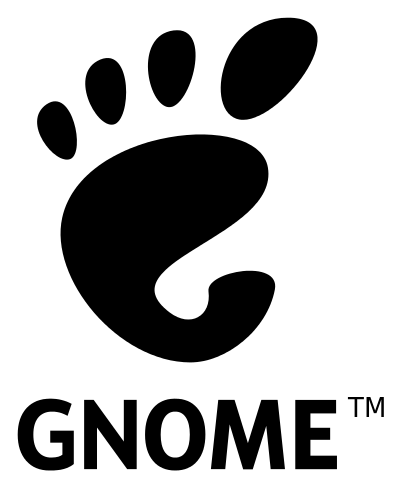
\includegraphics[scale=0.5]{images/Gnomelogo_svg.jpg}
%%  \end{figure}
%%\maketitle
\begin{document}
\makeatletter
\begin{titlepage}
  \centering
  \begin{figure}
    \centering
    \vspace{1cm}
    \textcolor{SteelBlue}{\fbox{\Huge{\emph{\textbf{Rapport de projet}}}}}\\
    % FireBrick, DarkRed, Indigo.
    \vspace{-5cm}
  \end{figure}


  \begin{figure}
    \centering
    \vspace{14cm}
          % FireBrick, DarkRed, Indigo.
          \vspace{2cm}
          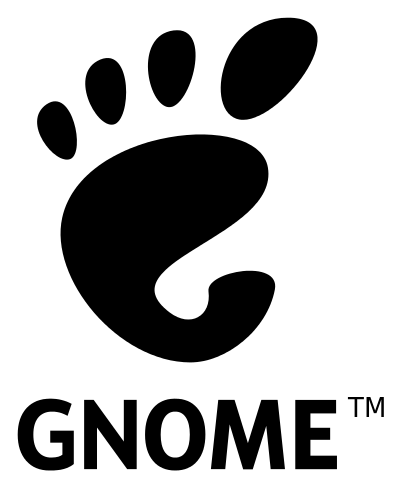
\includegraphics[scale=0.2]{images/Gnomelogo_svg.jpg}
    \vspace{-15cm}
  \end{figure}


  \begin{flushleft}
    \large{\textbf{Projet GNOME}} :\\{\@author}\\ 
    Licence ADSILLH\\
    Session 2017
  \end{flushleft}


  \vspace{15cm}
  %%\Large{Lycée Alfred Kastler}\\
  %%\normalsize{\textcolor{Peru}{14 Avenue de l'Université\\33402 Talence}}


  \vspace{-0.1cm}
  \centering
\includegraphics[scale=0.3]{images/logo_univ.jpg}
  
\end{titlepage}
\makeatother


\begin{abstract}
Ce document présente les différentes contributions effectuées dans le
cadre du projet sous licence libre de la licence ADSILLH.

Le but est avant tout de nous accoutumer au développement
collaboratif, et de nous apprendre à interagir avec une communauté
du logiciel libre.
\end{abstract}

\tableofcontents

%% % Useless
%% \chapter{Introduction}

%% \section{La Licence ADSILLH}
%% % from: http://dept-info.labri.fr/ENSEIGNEMENT/adsillh/contenu.html
%% L'objectif est de former des techniciens en informatique de haut
%% niveau en administration des systèmes d'information, polyvalents et
%% aptes à effectuer l'intégration de composants logiciels libres
%% appartenant à de nombreux domaines fonctionnels:
%% \begin{itemize}
%% \item systèmes d'exploitation
%% \item bases de données
%% \item serveurs web
%% \item téléphonie logicielle
%% \end{itemize}

%% alliant ainsi de solides compétences d'administration à des capacités
%% de développement, en partant des couches les plus basses jusqu'aux
%% plus hautes, et l'aptitude à intégrer ces développements au sein des
%% communautés libres. Ce profil est explicitement recherché par les
%% entreprises et fait l'unicité de la formation. Il est couramment
%% appelé « DevOps Engineer ».

%% La formation apporte également des aspects organisationnels en droit
%% et en économie des logiciels libres.

%% \section{Le projet}
%% Le but du projet est avant tout de nous accoutumer au développement
%% collaboratif, et de nous apprendre à intéragir avec une communauté
%% du logiciel libre.

\chapter{Le projet GNOME}
\section{Présentation}
% from: https://fr.wikipedia.org/wiki/GNOME
% Gautier : j'ai enlevé le terme ``environnement de bureau livre convivial'', ce n'est pas un terme objectif
% PA: L'objectivité existe t'elle ?
GNOME, acronyme de GNU Network Object Model Environment, est un
environnement de bureau libre  dont l'objectif est de rendre
accessible l'utilisation du système d'exploitation GNU au plus grand
nombre ; cette interface est actuellement populaire sur les systèmes
GNU/Linux et fonctionne également sur la plupart des systèmes de type
UNIX.

GNOME est développé par The GNOME Project dont les participants sont
bénévoles ou rémunérés par des entreprises externes au projet. La
majorité du travail est fournie par les contributeurs professionnels,
en premier lieu ceux travaillant pour Red Hat.

Dans ce document nous n'utiliserons pas forcément les noms complets des
projets, étant donné que nous somme dans le contexte de GNOME nous
simplifieront les noms en supprimant le terme GNOME.
Exemple: Gnome-Builder pourra être simplifié par Builder.

\section{Les outils collaboratifs} 
% TODO PA: Cette partie a besion d'une relecture ;)
\subsection{Bugzilla}
\label{bugzilla}
% from: https://fr.wikipedia.org/wiki/Bugzilla
Bugzilla est une solution de gestion de bugs, distribuée sous
% form: https://fr.wikipedia.org/wiki/Double_licence
tri-licence\footnote{Tri-licence: Le concept de licence multiple
  est de proposer un travail non pas sous une licence unique, mais
  en offrant un choix restreint de licence, pour permettre une plus
  grande flexibilité. (source:
  \href{https://fr.wikipedia.org/wiki/Licence_multiple}{Wikipedia})}
MPL\footnote{MPL: Mozilla Public License (source:
  \href{https://www.mozilla.org/en-US/MPL/}{Mozilla})}
/ GNU GPL\footnote{GNU GPL: GNU General Public License (source:
  \href{https://www.gnu.org/licenses/gpl.html}{Gnu})}
/ GNU LGPL\footnote{GNU LGPL: GNU Lesser General Public License (source:
  \href{https://www.gnu.org/licenses/lgpl.html}{Gnu})}
, elle est développée et utilisée à l'origine par Mozilla.
GNOME a mis en place un \href{https://bugzilla.gnome.org}{bugzilla} pour 
la gestion des bugs dans les différents projets.
%% (figure~\ref{figure_bugzilla} page~\pageref{figure_bugzilla})

%% \newline
%% % from: https://bugzilla.gnome.org/page.cgi?id=points.html
%% Bugzilla intègre aussi une fonctionnalité de "score"
%% %% (figure~\ref{figure_bugzilla_score} page~\pageref{figure_bugzilla_score})
%% , dont le but est a l'origine d'avoir une idée 
%% aproximative de l'activité d'une personne  sur le bugzilla, et donc 
%% des personnes qui sont le plus experimenté pour aidée les autres 
%% utilisateurs. Mais ce dispositif s'est revelé peu efficace. Le
%% score est donc plus une fonctionnalite un peut fun qu'un vrai outils.
%% A noter qu'il existe quand même un classement de la semaine, disponible 
%% \href{https://bugzilla.gnome.org/page.cgi?id=weekly-bug-summary.html}{ici}.

\subsection{Wiki}
\label{wiki}
GNOME dispose d'un \href{https://wiki.gnome.org/}{wiki} où l'on peut retrouver 
les documentations sur les différents projets.
%% (figure~\ref{figure_wiki} page~\pageref{figure_wiki}).

\subsection{Git}
\label{git}

\label{cgit}
Le projet GNOME dispose de plusieurs interfaces Git. L'interface 
principale est basée sur le logiciel libre "cgit"
%% (figure~\ref{figure_cgit} page~\pageref{figure_cgit})
, on peut y retrouver la plupart des projets GNOME 
(\href{https://git.gnome.org/}{ici}). Pour créer un bug il faut passer par Bugzilla
(section~\ref{bugzilla}).

\label{gitlab}
GNOME a aussi mis en place un \href{https://gitlab.gnome.org/GNOME}{GitLab} 
ou l'on peut trouver de nombreux projets. L'interface est plus moderne,
par exemple nous pouvons créer des "Pull Requests" comme sur github
et le report de bug est sur l'interface gitlab, donc pas besoin de passer
par le Bugzilla. Il est aussi possible de parcourir le code via l'interface
web de gitlab.
%% (figure~\ref{figure_gitlab} page~\pageref{figure_gitlab}).

\label{github}
Il existe aussi un miroir des répertoires git des projets 
\href{https://github.com/GNOME}{GNOME sur GitHub}.

\subsection{IRC}
Le projet GNOME dispose aussi d'un chat irc (\href{irc.gnome.org}{irc.gnome.org})
avec de nombreux salons, dont voici quelque exemples :
\begin{itemize}
\item \#gnome-hacker : Pour les dicussions sur le développement de GNOME ;
\item \#newcomers : Pour les nouveaux contributeurs au projet ;
\item \#gnome-games : Pour les discutions autour du projet Games ;
\item \#vala : Spécifique pour le language vala.
\end{itemize}

\subsection{Mailing lists}
Des mailing lists sont aussi à notre disposition pour se tenir informer.
% PA: TODO Useful ?

\subsection{Newcomers}
Le projet GNOME met à disposition sur son site un guide pour les nouveaux
arrivants souhaitant contribuer au projet.Cette section nous propose
tout d'abord le chat irc dédié aux nouveaux contributeurs, ainsi que la
mailing list qui leur ai réservée
(\href{https://mail.gnome.org/mailman/listinfo/newscomers-list}{ici}).

Quelques conseils sont aussi donnés: patience,respect des autres et prise
d'initiatives sont des qualités nécessaires au bon fonctionnement du projet.

Il est ensuite présenté Flatpack qui permet d'installer Builder.
C'est un environnement de développement intégré qui permet de travailler
sur les applications GNOME. Il permet de télécharger les sources d'un
projet et de pouvoir travailler dessus et de le construire grâce à une
interface graphique simplifiée. Il permet en effet d'éditer des fichiers
ou de compiler le projet avec un seul bouton, de gérer les dépendances
et met à disposition un débogueur

On nous présente ensuite la documentation disponible sur
\href{https://developper.gnome.org/search} ainsi que sur la page du
projet concerné. On nous explique ensuite que chaque projet possède
des bugs dédiés aux newcomers. Ce sont des bugs qui permettent aux
nouveaux arrivants de se familiariser à la fois avec le code et
avec la manière de corriger un bug grâce à des bugs pas trop
complexe.

Le guide aiguille ensuite le nouvel arrivant sur la façon de corriger
un bug en comprenant ce qu'il se passe et en changeant le code de
façon à le corriger. Enfin le guide nous montre comment créer un
patch depuis le commit et le poster sur le bug report sur bugzilla.


\newpage
\chapter{GNOME-Music}
GNOME Music est une application permettant d'écouter de la musique, 
son interface se veut particulièrement simple afin de permettre aux
utilisateurs de gérer facilement leur musique, leur bibliothèques, 
les recherches et la lecture de leur fichiers audio.
Les sources du projet sont disponibles sur github :
\href{https://github.com/GNOME/gnome-music}{ici}

\section{Architecture du projet}
% TODO 

\section{Le langage Python}
% https://fr.wikipedia.org/wiki/Python_(langage)
Le projet est écrit dans le langage Python. C'est un langage de
programmation objet, multi-paradigme et multiplateformes. Il favorise la
programmation impérative structurée, fonctionnelle et orientée objet. 
Il est doté d'un typage dynamique fort, d'une gestion automatique de la 
mémoire par ramasse-miettes et d'un système de gestion d'exceptions ; 
il est ainsi similaire à Perl, Ruby, Scheme, Smalltalk et Tcl.

Python est un langage qui peut s'utiliser dans de nombreux contextes 
et s'adapter à tout type d'utilisation grâce à des bibliothèques 
spécialisées. Il est cependant particulièrement utilisé comme 
langage de script pour automatiser des tâches simples mais 
fastidieuses, comme un script qui récupérerait la météo sur Internet 
ou qui s'intégrerait dans un logiciel de conception assistée par 
ordinateur afin d'automatiser certains enchaînements d'actions 
répétitives (voir la section Adoption). On l'utilise également comme 
langage de développement de prototype lorsqu'on a besoin d'une 
application fonctionnelle avant de l'optimiser avec un langage 
de plus bas niveau. Il est particulièrement répandu dans le monde 
scientifique, et possède de nombreuses extensions destinées au 
calcul numérique.

Python a été conçu pour être un langage lisible. Il vise à être 
visuellement épuré. Par exemple, il possède moins de constructions 
syntaxiques que de nombreux langages structurés tels que C, 
Perl, ou Pascal. Les commentaires sont indiqués par le caractère 
croisillon (\#).

Les blocs sont identifiés par l'indentation, au lieu d'accolades 
comme en C ou C++ ; ou de begin ... end comme en Pascal ou Ruby. 
Une augmentation de l'indentation marque le début d'un bloc, et 
une réduction de l'indentation marque la fin du bloc courant. 

\section{Premiers pas avec le projet}
\subsection{Compilation 1ere Partie}
Lorsque nous avons voulu compiler le projet nous avons rencontré 
beaucoup de problèmes notamment ceux liés aux dépendances nécessaires
à la compilation. Ces dépendances là ne sont pas indiquées dans la
documentation et nous devions alors les installer une par une à
mesure ou nous ne pouvions nous rendre compte des dépendances 
manquantes que lors de la compilation. 
Nous avons ensuite eu un problème avec le paquet libtracker-sparql
qui bien qu'étant installé n’était pas considéré comme tel.

\subsection{GNOME Builder}
Nous sommes ensuite passé sur GNOME Builder pour compiler le projet.
En effet grâce à cet environnement de développement intégré les 
dépendances sont gérées automatiquement. Cependant là aussi nous
avons rencontré des problèmes tout d'abord car les téléchargements
réalisés par GNOME Builder était trop gros pour nos VM puis nous 
nous avons rencontré un bug lors de l’exécution de l'application.
En effet lors de l'exécution de celle-ci depuis le builder l'application
ne s'affichait pas correctement, il n'y avait pas les boutons en haut
et le répertoire de musique n’était pas trouvé. Cela nous a mené à 
faire notre premier rapport de bug(Voir ci-après).

\subsection{Compilation 2eme Partie}
Nous étions alors sur Ubuntu depuis le début du projet et nous avons
décidé de passer sur debian sans utiliser GNOME Builder afin d'avoir 
une compilation plus facile. Ce fut le cas grâce notamment à la 
commande build-dep qui permet de récupérer toutes les dépendances d'un 
projet. Nous avons donc pu commencer à travailler sur projet en 
lui-même.

\section{Bug reports}
% TO DO

\newpage
\chapter{GNOME-Games} %% Change GNOME-Games to Games ?
Games est une application permettant la gestion d'une
bibliothèque vidéoludique. Elle est capable de s'interfacer avec de
nombreux émulateurs.

Au début du projet Games étais disponible sur le git de GNOME, mais 
depuis peut il a migré sur Gitlab.

\section{Les projets associés}
Le projet s'appuie sur plusieurs autre projets:
\begin{itemize}
\item retro-gtk : Développé pas le mainteneur de Games et utilisant les bibliothèques libretro,
retro-gtk permet à Games de lancer les jeux retro.
\item libmanette : Libmannette et aussi développé pas le mainteneur de Games. Cette bibliothèque
permet la gestion des manettes.
% TODO Verifier les info pour libmanette et retro-gtk 
\end{itemize}

\section{Le langage Vala}
% from: https://fr.wikipedia.org/wiki/Vala_(langage)
Vala est un langage de programmation compilé, dont l'objectif est de
fournir les bénéfices des langages de programmation modernes (comme la
POO) aux développeurs de la plateforme GNOME qui utilisent GLib et son
système GObject.

Sa syntaxe est basée sur celle de C\# mais il ne nécessite pas
d'environnement d'exécution. Vala est transformé en code C, lui-même
compilé en code machine natif. Les avantages d'une telle chaîne de
compilation sont de produire des logiciels qui requièrent moins de
mémoire vive et qui s'exécutent plus rapidement.

De plus, ce passage par l'étape C rend possible l'utilisation des
bibliothèques C au moyen d'interfaces définies dans les fichiers
Vapi. Des fichiers Vapi sont fournis avec Vala pour une grande partie
de la plateforme GNOME, ainsi que pour d'autres bibliothèques.

\section{Le format Flatpak}
% from: https://fr.wikipedia.org/wiki/Flatpak
Flatpak, nommé xdg-app jusqu’en mai 2016, est un système de
virtualisation d’application pour les distributions GNU/Linux de
bureau.

L'objectif est de fournir un environnement « bac à sable » (sandbox)
sûr, isolé du reste du système, dans lequel les utilisateurs peuvent
exécuter des applications non validées par les dépôts de la
distribution (des versions de test, par exemple). Les applications
utilisent des appels de fonctions spécifiques fournies par xdg-app
pour contrôler les périphériques matériels ou accéder aux fichiers de
l'utilisateur, et xdg-app demande à l'utilisateur sa permission avant
de donner accès.

Le nom originel vient de freedesktop.org, qui est souvent abrégé en «
xdg », cette structure ayant hébergé sur ses serveurs le projet
xdg-app. En mai 2016, le projet a été rebaptisé « Flatpak ».

En juin 2016, un certain nombre d'applications connues sont portées en
format Flatpak, comme MonoDevelop, GNOME Shell, Pitivi ou LibreOffice.

Les applications Flatpak se téléchargent sous forme d'un fichier qui
peut s’exécuter directement sur le système, de façon indépendante de
la distribution Linux précise utilisée, sous réserve que le logiciel
Flatpak ait été préalablement installé sur cette distribution.

Pour permettre au « bac à sable » de fonctionner malgré son isolement
du système, il faut donc que les bibliothèques ou dépendances
indispensables à un logiciel soient embarquées avec lui au sein de son
paquet « Flatpak ». Ce système a pour inconvénient d'embarquer
potentiellement plusieurs fois la même bibliothèque (une par paquet
Flatpak), et donc de prendre plus de place. Il a par contre pour
avantage de ne pas déstabiliser un logiciel Flatpak lors d'une mise à
jour de dépendances ou de bibliothèques, puisque cette mise à jour ne
le concernera pas. Il est dès lors assez simple de faire cohabiter
plusieurs versions d'un même logiciel.

\section{Découverte du logiciel}
\subsection{Compilation}
Nous avons rencontrés de nombreux problèmes relatifs à la compilation,
cela étant en grande partie dû à l'utilisation de bibliothèques encore en
état de développement actif, ainsi qu'au système de configuration
``Meson'' qui est un remplacement de ``./configure''.

Ainsi il a été nécessaire de compiler certaines librairies, parmi
lesquelles\footnote{Nous avons utilisé Debian Sid comme OS de développement et de test}:
\begin{itemize}
\item retro-gtk
\item libmanette
\end{itemize}

De plus, aucun fichier ne documentait la procédure d'installation,
cela nous à particulièrement posé problème car nous ne nous
connaissions pas le système de build 'Meson'.

Nous avons aussi tenté d'utiliser l'IDE Gnome-Builder, qui possède une
fonctionnalité permettant de télécharger automatiquement les
dépendances.

Cependant nous n'avons pas réussi à l'utiliser sur la branche master,
car il ne pouvait pas trouver les bonnes librairies.

Lors de l'utilisation de Games, nous avons rencontrés quelques
problèmes, certains jeux étaient chargés avec de mauvaises jaquettes,
et il était impossible de paramétrer les touches du clavier.

\section{Les bug reports}
% Gautier : système de statuts -> aucune explication
% Gautier : lecture de différents bug reports, et réécriture plus simple dans un
%           fichier partagé pour effectuer un premier tri
\subsection{Bug PulseAudio}
Un bug avec PulseAudio était déclaré pour Games, en effet le programme crashait
quand le serveur PulseAudio était éteint et que l'on tentait de lancer
un jeu.

Il a donc fallu reproduire le bug, pour cela nous avons personnalisé notre
configuration PulseAudio pour qu'elle ne se relance pas automatiquement.
\begin{minted}[breaklines]{console}
/etc/pulse/client.conf:
   autospawn = no
\end{minted}

Nous avons aussi utilisé une commande pour simuler le crash du serveur PulseAudio.
\begin{minted}[breaklines]{console}
  $ PulseAudio --kill
\end{minted}

Le terminal retournait le message d'erreur suivant:
\begin{minted}[breaklines]{console}
Assertion 'p' failed at pulse/simple.c:273, function pa_simple_write(). Aborting.
\end{minted}

En vérifiant dans les sources de PulseAudio on retrouve bien l'``assert'' qui provoque
l’arrêt prématuré du programme.
\begin{minted}[breaklines]{c}
  pa_assert(p);
\end{minted}

A partir de là nous avons tracé le bug dans le code source de gnome-games et retro-gtk.
Pour cela nous avons commencé par utiliser la commande ``git grep'' pour retrouver
la (ou les) fonction(s) susceptible d'appeler ``pa\_simple\_write ()''.
\begin{minted}[breaklines]{console}
$ git grep ``pa_simple_write''
\end{minted}

Aucune fonction n'a été trouvée dans les sources de Games, par contre il y a bien
une fonction qui fait appel à ``pa\_simple\_write'' dans retro-gtk.
Nous avons donc pu déterminer que la fonction
``retro\_pa\_player\_on\_audio\_output'' (définie dans le fichier
``retro\_pa\_player.c'' du projet ``retro-gtk'') appelle la fonction de PulseAudio
``pa\_simple\_write'' qui provoque le crash.

\begin{minted}[breaklines]{c}
  if (self->simple == NULL || sample_rate != self->sample_rate)
    retro_pa_player_prepare_for_sample_rate (self, sample_rate);

  pa_simple_write (self->simple, data, sizeof (gint16) * lenght, NULL);
\end{minted}
  
Après quelques test et une vérification dans les sources nous  avons compris
que la fonction ``retro\_pa\_player\_prepare\_for\_sample\_rate'' retourne ``self''
équale à ``NULL'' si PulseAudio n'est pas disponible.

La solution la plus simple était de contourner la fonction ``pa\_simple\_write''
avec un test de la valeur de la structure et un ``return'' prématuré dans la fonction
appellante si la valeur est ``NULL''. Nous avons aussi pensé à afficher un message à
l'utilisateur et luis demandant si il voulais lancer quand même le jeux mais sans le son.

La premiere solution nous a parut trop simple et pas suffisament fiable, et la
seconde un peu trop compliquée à mettre en oeuvre sur un projet que l'on découvrait juste.
Nous avons donc décidés de poster sur le rapport de bug notre analyse du problème, et
d'attendre une décision du mainteneur.

Finalement le mainteneur a opté pour la première solution et a ajouté un test, comme
ci-desous:
\begin{minted}[breaklines]{c}
  if (self->simple == NULL || sample_rate != self->sample_rate)
    retro_pa_player_prepare_for_sample_rate (self, sample_rate);

  if (self->simple == NULL)
    return;

  pa_simple_write (self->simple, data, sizeof (gint16) * lenght, NULL);
\end{minted}

\section{Nos patchs}
% TODO PA: Cette partie a besion d'une relecture
\subsection{Mise à jour du fichier HACKING}
Le premier patch que nous avons envoyé est en réponse à un bug report
(\href{http://bugzilla.gnome.org/show_bug.cgi?id=788692}{ici}), il ajoute une
aide pour la compilation du projet.

Il n'y avait aucune aide ou information dans la documentation sur la compilation
du projet. Étant nouveaux dans le projet GNOME nous n'avions pas connaissance de 
Builder qui permet assez simplement de construire le projet. Mais même avec cet
outil, la compilation s'est revélée ardue. En effet le fonctionement de Builder a
tendance à changer entre les versions et certaines actions comme un ``git pull''
peuvent poser problème. Nous avons donc désidé de modifié le fichier HACKING du
projet pour y ajouter des instruction de compilation.

Le projet utilise pour le moment le système ``autotools'' pour sa configuration et 
sa compilation, mais pour la version 2.30 il est prévu qu'il passe à un système
avec le logiciel ``meson'' pour la configuration.

Après des recherches et un peu d'aide, nous avont réussi à avoir une procédure
complète pour la compilation du projet. L'une des difficultés que l'on peut
rencontrer pour la compilation de Games et qui est le sujet du bug report sur le
quelle nous avons répondu, est le fait que la version master de Games a besoin de
la version master de ``retro-gtk'' et ``libmannette''. Cette spécificité n'est
indiqué nulle part dans la documentation et les dépendances de ces deux
bibliothèques ne sont pas à jour dans la liste de dépendances d'autotools.

Nous avons nous-même rencontrés des problèmes de compilation, il nous a donc
semblé important de donner des indications pour que les prochaines personnes qui
voudraient contribuer ne soient pas freinées par un problème comme celui-ci.

Il y a eu de nombreux ajustements demandés par le mainteneur, notament la demande
d'utilisation de la syntaxe Markdown. D'autres parties de notre patch original se sont
revélées peu utiles ou pratiquement impossibles à maintenir. Nous voulions par
example faire une liste exhaustive des dépendances du projet, cette idée a été
refusée par le mainteneur car très difficile a maintenir d'une version à l'autre.
Après plusieurs modifications et échanges avec le mainteneur le patch a été
accepté et commité.

\subsection{Mise à jour du fichier README.md}
Le second patch (\href{http://bugzilla.gnome.org/show_bug.cgi?id=790454}{ici}) 
que nous avons envoyés, est une mise à jour de la documentation de retro-gtk.
En effet retro-gtk est passé d'un système de compilation 'autotools' à un
système avec le logiciel 'meson' et le compilateur 'ninja'.
Nous avons donc mis à jour le fichier README.md en respectant la syntaxe
'Marckdown', utilisé par github et gitlab par exemple.
Le patch n'a pas encore été accepté.

\subsection{Retour à la collection avec les touches Alt+Left}
Le but de ce patch est de lier un évent à une combinaison de touches
(en l’occurrence Alt+Left).

La modification a consisté à modifier un fichier, celui-ci se trouvait
dans le répertoire /src/ui et se nommait application-window.vala .

Une fonction permettant de retourner à la collection existait déjà:

\begin{minted}[breaklines]{vala}
private void on_display_back () {
  if (quit_game ())
  ui_state = UiState.COLLECTION;

  uninhibit (Gtk.ApplicationInhibitFlags.IDLE | Gtk.ApplicationInhibitFlags.LOGOUT);
}
\end{minted}

Une fonction qui liait l'appui de certaines touches à des événements
était aussi déjà présente:

\begin{minted}[breaklines]{vala}
  private bool handle_display_key_event (Gdk.EventKey event) {
    if (ui_state != UiState.DISPLAY)
    return false;

    var default_modifiers = Gtk.accelerator_get_default_mod_mask ();

    if ((event.keyval == Gdk.Key.f || event.keyval == Gdk.Key.F) &&
    (event.state & default_modifiers) == Gdk.ModifierType.CONTROL_MASK &&
    display_header_bar.can_fullscreen) {
      is_fullscreen = !is_fullscreen;
      settings.set_boolean ("fullscreen", is_fullscreen);

      return true;
    }

    if (event.keyval == Gdk.Key.F11 && display_header_bar.can_fullscreen) {
      is_fullscreen = !is_fullscreen;
      settings.set_boolean ("fullscreen", is_fullscreen);

      return true;
    }

    if (event.keyval == Gdk.Key.Escape && display_header_bar.can_fullscreen) {
      is_fullscreen = false;
      settings.set_boolean ("fullscreen", false);

      return true;
    }
    
    return false;
  }
\end{minted}

C'est en prenant cet extrait pour exemple que nous avons ajouté une
condition dédiée à Alt+Left, il nous a été nécessaire de chercher dans
la documentation du langage Vala pour trouver la X (modifier key ?)
correspondante.

Voici le code correspondant à notre patch:

\begin{minted}[breaklines]{vala}
  if (event.keyval == Gdk.Key.Left){			
    on_display_back ();
    
    return true;
  }
\end{minted}

Puis en effectuant des tests, nous nous sommes rendus compte que la
condition validant l'appui sur la touche Alt n'était pas nécessaire;
pourtant, le déclenchement de l'évent nécessitait toujours un appui
physique sur Alt.

Par la suite, le mainteneur à décidé de réécrire le patch pour ajouter
la vérification de la pression sur la touche Alt:

\begin{minted}[breaklines]{vala}
  if (((event.state & default_modifiers) == Gdk.ModifierType.MOD1_MASK) &&
  (((get_direction () == Gtk.TextDirection.LTR) && event.keyval == Gdk.Key.Left) ||
  ((get_direction () == Gtk.TextDirection.RTL) && event.keyval == Gdk.Key.Right))) {
    on_display_back ();

    return true;
  }
\end{minted}

%% % Annexe:
%% \appendix
%% \chapter{GNOME en images}

%% \begin{figure}[p]
%%   % from: https://bugzilla.gnome.org
%%   \caption{\label{figure_bugzilla} Le bugzilla du projet GNOME}
%%   \includegraphics[width=15cm]{images/bugzilla_gnome_org.png}
%% \end{figure}

%% \begin{figure}[p]
%%   % from: https://bugzilla.gnome.org
%%   \caption{\label{figure_bugzilla_score} Score sur bugzilla}
%%   \includegraphics[width=5cm]{images/score.png}
%% \end{figure}

%% \begin{figure}[p]
%%   % from: https://wiki.gnome.org
%%   \caption{\label{figure_wiki} Le wiki du projet GNOME}
%%   \includegraphics[width=15cm]{images/wiki_gnome_org.png}
%% \end{figure}

%% \begin{figure}[p]
%%   % from: https://git.gnome.org
%%   \caption{\label{figure_cgit} Interface git du projet GNOME}
%%   \includegraphics[width=15cm]{images/git_gnome_org.png}
%% \end{figure}

%% \begin{figure}[p]
%%   % from: https://gitlab.gnome.org
%%   \caption{\label{figure_gitlab} Le gitlab du projet GNOME}
%%   \includegraphics[width=15cm]{images/gitlab_gnome_org.png}
%% \end{figure}

%% \chapter{Patchs} 
%% % PA: Utile ? 

\end{document}
